\documentclass[11pt]{article}
\usepackage{graphicx}
\usepackage{amssymb}
\usepackage{amsmath}
\usepackage[backend=bibtex,style=ieee,bibencoding=ascii,sorting=none]{biblatex}
\usepackage{fancyhdr}
\usepackage{geometry}
\usepackage[export]{adjustbox}
\usepackage{subcaption}
\usepackage{hyperref}

\geometry{left=0.5in, right=0.5in, top=1in,bottom=0.5in}
\pagestyle{fancy}
\fancyhf{}
\fancyhead[L]{Carlos Martinez-Villar}
\fancyhead[C]{STAT 9100}
\fancyhead[R]{Final Project Report}
\title{Final Project Report\\STAT 9100 - Statistical Learning with Networks}
\author{Carlos Martinez-Villar}
\date{\today}
\addbibresource{refs}


\begin{document}
	%\maketitle
	%%%%%%%%%%%%%%%%%%%%%%%%%%%%%%
	% INTRODUCTION
	%%%%%%%%%%%%%%%%%%%%%%%%%%%%%%
	\section{Introduction}
	The present report discusses Hopfield networks (HNs) and some of their properties in relation to the subjects presented throughout this semester as an additional model of a network that can learn. Section \ref{model} includes a somewhat detailed description of the Hopfield model. 
	The first subsection therein describes the equations and rules that were enough to implement a simple version of this model and make it work.
	The last subsection (\ref{other}) includes a broader discussion of these models' context with analogies to statistical physics and the Ising model. 
	Section \ref{experiments} includes details on the implemented model and its shortcomings. 
	
	%%%%%%%%%%%%%%%%%%%%%%%%%%%%%%
	% MODEL
	%%%%%%%%%%%%%%%%%%%%%%%%%%%%%%
%	\cite{hebb2005organization}
%	\cite{mackay2003information}

	\section{Hopfield's Model and Approach to the Project}\label{model}
	
	The bulk of the method used here was proposed early on by Hopfield in \cite{hopfield1982neural}  and \cite{hopfield1984neurons} as a system consisting of individual nodes that–despite being very simple individually–showed collective properties with representational power. 
	This collective representational power was higher than the individual representational power of the constituent elements, so the system was capable of storing a system-wide state based on individual elements' states. 
	
	This relation between individual and collective states was analogous–as Hopfield noted–to physical systems where ``interactions among a large number of elementary components yield collective phenomena such as stable magnetic orientations [...] or vortex patterns in fluid flow". 
	Since his goal was to find a comparable collective computational phenomenon that could arise from a set of neurons, he considered that finding a stable system state (i.e.: an attractor) must be akin to categorizing a general concept or \textit{gestalt}, and/or correctly storing and retrieving a memory.
	
	Hopfield initially proposed this model as a content-adressable memory which is–basically–any storage system that can find data from a partially matching search term given to it.
	Thus the solution given in the original paper was presented as a network that could (i) learn a pattern and (ii) converge to a closest pattern when shown a partial pattern. 

	\subsection{Model Specification} 
	Haykin \cite{haykin} describes HNs, within the grand realm of neural networks, as a neurodynamic recurrent network with a \textit{global feedback}. 
	This is quite different from neural networks commonly used nowadays \cite{deeplearning2015} which have a clear forward and backward direction.
	The feedback property can be appreciated through the diagrams in figure \ref{fig:net} which shows a Hopfield network with 4 neurons. 
	Figure \ref{fig:netcircuit} shows the commonly used circuit diagram for a Hopfield network, and figure \ref{fig:netgraph} shows an equivalent graph similar to those studied throughout the semester. 
	The latter diagram is equivalent to the former if we assume that a single edge in figure \ref{fig:netgraph} is equivalent to two directed edges in either direction in figure \ref{fig:netcircuit}. 
	More formally, if $w_{ij}$ is the connection strength between nodes (neurons) $i$ and $j$, then $w_{ij} = w_{ji}$.



	%%%%%%%%%%%%%%%%%%%%%%%%%%%%%%
	% V UPDATE
	%%%%%%%%%%%%%%%%%%%%%%%%%%%%%%
	\subsubsection{Update Rule for the State of a Node}
	The original model introduced by Hopfield in \cite{hopfield1982neural} considered binary states for each neuron, so we can let $x_j \in \{ -1, 1 \}$ be the state of a node $j$ for $j=1,\ldots ,N$ in a network of $N$ neurons.
	Setting a simple rule that will determine the state of each node must be based on the fact that each node must change its state according to an input defined by the nodes connected to it. 
	In this case the neighborhood of this node will be all other nodes.
	If we let $W$ be a matrix of node interactions containing the edge weights $w_{ij}$, then we can determine the individual state of a node $x_j$ by using equation \ref{eq:nodeupdate}.
	
	\begin{equation} \label{eq:nodeupdate}
		x_j = \begin{cases}
			 -1  & \text{if } \sum^{N}_{i \neq j} x_i W_{ij}  < -b_j \\
			1  & \text{if } \sum^{N}_{i \neq j} x_i W_{ij} \ge -b_j
		\end{cases}
	\end{equation}
	
	Provided with this equation each node $j$ will set its state to -1 or 1 based on the nodes $i$ connected to it. 
	Each input $i$ is multiplied by the connection strength $w_{ij}$, and the sum coming from all the $i$ nodes is either above or below a given threshold. 
	In the implementations shown in section \ref{experiments} the threshold $-b_j$ is set to zero.



	%%%%%%%%%%%%%%%%%%%%%%%%%%%%%%
	% T UPDATE
	%%%%%%%%%%%%%%%%%%%%%%%%%%%%%%	
	\subsubsection{Storing a Pattern}
	If we would like the network to recall a pattern, we must set a rule for the edges to learn this pattern we want to store. 
	We can set the value for an edge according to the agreement between two nodes (i.e.: being in the same state or not). 
	To store all, we have to define a weight matrix  $W$ with edge weights $w_{ij}$ in it.This agreement or disagreement is represented by positive or negative numbers as
	
	\begin{equation}\label{eq:weights}
	\begin{cases}
		W_{ij} > 0 \ \text{between nodes $i$ and $j$ in the same state}\\
		W_{ij} < 0 \ \text{otherwise}
	\end{cases}
	\end{equation}
	
	At this point we can determine each edge $w_{ij}$. 
	In other words, provided we have a pattern we wish to store, we can let the network adjust and find an appropriate set of weights to recall that state. 
	Once the matrix $W$ is set, we can feed the network anything and expect it to recover the pattern that was used to set $W$. 

	%%%%%%%%%%%%%%%%%%%%%%%%%%%%%%
	% T AVERAGE
	%%%%%%%%%%%%%%%%%%%%%%%%%%%%%%
	\subsubsection{Storing Multiple Patterns}
	Similarly, we can find a connection matrix $W$ that works for a set of multiple patterns (memories) instead of a single one.
	 One way to store multiple such memories in a network is to follow the average co-activation between nodes over the set of memories. 
	 This is perhaps arbitrary but was Hopfield's original prescription in \cite{hopfield1982neural} written as $\Delta W_{ij} = [X_i(t) X_j(t)]_{average}$, where the delta would be change over $t$ as a ``past history".
	 We can set this as follows. Since the state of our HN consists of individual binary states, we can represent the overall state of the network with a binary vector. 
	 Let $X^{(s)}$ be a binary vector of size $N$ representing a state $s$ for our network of $N$ neurons.  
	 Taking our past history of $M$ memories to be the set of states  $\{ X^{(1)}, \ldots, X^{(M)} \}$, then
	\begin{equation}\label{eq:weightupdate}
		W_{ij} = \frac{1}{M} \sum^{M}_{s=1} X^{(s)}_i X_j^{(s)}, \ \ i \neq j
	\end{equation}
	With equation \ref{eq:weightupdate} our usual adjacency matrix is set to a co-activaction matrix with $W_{ij}$'s that are the \textit{average co-activation between nodes} $i$ and $j$. There are no self-connected nodes, so $W_{ii} = 0$. 
	This is can be written in vector form as
	\begin{equation}
	W = \frac{1}{M} \sum^{M}_{s=1} X^{(s)} {X^{(s)}}^T - I
	\end{equation}
	where $I$ is the identity matrix substracting the resulting ones of a node with itself to set $W_{ii} = 0$.
	
	%%%%%%%%%%%%%%%%%%%%%%%%%%%%%%
	% E
	%%%%%%%%%%%%%%%%%%%%%%%%%%%%%%	
	\subsubsection{Hopfield's Energy}
	The most interesting concept in HNs–and perhaps the one that pertains the subject of this course the most–was the concept of Hopfield energy. 
	The overall energy of the system is the sum of the contributions of each node. 
	In turn, each node contribution depends on its connection to other neurons $W_{ij}$ and the state of these neurons. 
	Take the network to be presently at any state $\mathbf{s}$ (to distinguish it from the memories $X$ used to set $W$) and let $s_i$, $s_j$ be elements in $\mathbf{s}$ corresponding to nodes $i$ and $j$. 
	Each contribution depends on one connection weight and the states of two neurons, so the total energy of the system at any time is defined as	
	\begin{equation}\label{eq:energy}
		E = - \frac{1}{2}\sum^{}_{j \neq i}  \sum^{}_{i \neq j}  s_j s_i W_{ij} - \sum^{}_{j} s_j b_j
	\end{equation}
	This energy is analogous to potential energy in the sense that a stabler state represents a lower energy level.
	The bias term for a node $j$ is set to the average node activation over all memories, i.e.: $b_j = \sum^{M}_{s=1} X_j^{(s)}$. 
	The intution behind $b_j$ is that if a node $j$ is on it reduces $E$ by $b_j$. If it is off, it will increase $E$ by $b_j$. 
	Similarly, the product of $s_i$ and $s_j$ will have a sign depending on the state of these nodes. 
	The nodes will decrease $E$ if their product matches our pre-defined $W_{ij}$, and increase it otherwise. 
	The whole interaction term is divided by two to avoid double counting, which can also be written as an indexing over  $i < j$ (upper or lower triangular matrix) without the fraction.
	Equation \ref{eq:energy} can be re-written in a more convenient matrix form as
	\begin{equation}\label{eq:energymatrix}
		E = -\frac{1}{2}\mathbf{s}^T W\mathbf{s} - \mathbf{s}^T \mathbf{b}	
	\end{equation}
	

	%%%%%%%%%%%%%%%%%%%%%%%%%%%%%%
	% GRADIENTS
	%%%%%%%%%%%%%%%%%%%%%%%%%%%%%%	
	\subsubsection{Relation to Gradient Descent}
	Gradient descent–or rather stochastic gradient descent and its newer flavors–is the most commonly used method for optimizing neural networks \cite{deeplearning2015}.
	Even though HNs are siginificantly different from other models, it is pleasing to see that they can be described as a gradient optimization problem as well, unifying the theory. 
	Taking the gradient of the energy function for a particular node gives
	
	\begin{equation}\label{eq:partialnode}
		\frac{\partial E}{\partial X_j} = - \sum^{}_{i} X_i W_{ij} - b_j
	\end{equation}
	
	This is the  "$\Delta E$ due to $\Delta X_i$" described by Hopfiled \cite{hopfield1982neural}. Taking the derivative of energy with respect to the weights gives
	
	\begin{equation}\label{eq:partialweights}
		\frac{\partial E}{\partial W_{ij}} = - X_i X_j
	\end{equation}

	And hence, equations \ref{eq:partialnode} and \ref{eq:partialweights} agree with equations \ref{eq:nodeupdate} and \ref{eq:weightupdate}. 
	An alternative way to think of equation \ref{eq:partialnode} is to see the difference in energy between on and off for a particular node (energy gap):
	
	\begin{equation}
		\Delta E_j = E(X_j = 0) - E(X_j = 1) = b_j + \sum^{}_{i}X_i W_{ij}
	\end{equation}

	%%%%%%%%%%%%%%%%%%%%%%%%%%%%%%
	% OTHER
	%%%%%%%%%%%%%%%%%%%%%%%%%%%%%%	
	\subsection{Relationship to Other Models}\label{other}

	% ISING
	%%%%%%
	\subsubsection{Ising's Model and Statistical Physics}\label{ising}
	Hopfield, in \cite{hopfield1982neural}, recognized the link between his content-addressable approach and the Ising model. 
	The most obvious parallel is that nodes in a HN can be considered a dipole. 
	In a broader sense though, any node is affected by its neighbors and its neighbors are affected by a node. 
	A HN system, just like Ising's model, will reach a solution at a point when any single flip of a dipole will increase the energy of the system. 
	The Ising lattice model will snap up and down until any change will increase energy instead of decreasing energy, just like a Hopfield model will consistently minimize potential energy to reach a lower state. 
	The HN is clearly unstable in similar fashion to Ising's: if we pick a dipole at random and flip it, it could cause a cascade of flips.
	And if we repeatedly pick a node at random and flip it, in large set of models, we should be able to reach a \textit{stable proportion of models in each given state} in a way comparable to thermal equilibrium.

	% RBMs
	%%%%%%%
	\subsubsection{Boltzmann Machines and a Possible Exhaustive Computation}\label{boltzmann}
	As shown in \cite{hinton2012practical}, the probabilty that a unit $i$ is on in a Boltzmann machine is 
	\begin{equation}\label{eq:hopfieldtemperature}
		P(s_i=1) = \frac{1}{1 + e^{-\Delta E_i / T} }
	\end{equation}
	Which is simply a logistic activation function for a node and a "temperature" term $T$. 
	Just like a Heaviside step function can be turned into a logistic one, so we can define the binary threshold function of Hopfield in terms of a logistic function. 
	When the $T \rightarrow 0 $, the exponential term approaches $-\infty$ or $\infty$ based solely on the sign of $\Delta E_i$.
	
	Given that HNs are special case of a Boltzmann Machine, we can then borrow some concepts that make it possible to derive a probability distribution. The probability of a state $i$ in Boltzmann machine is
	
	\begin{equation}\label{eq:rbm}
		p(v,h) = \frac{1}{Z} e^{-E(v,h)}
	\end{equation}
	
	 Where $Z$ is the partition function. The Boltzmann distribution is
	
	\begin{equation}
		p_i = \frac{1}{Z} e^{-E_i/T}
	\end{equation}
	 
	In equation \ref{eq:rbm} $v$ and $h$ are visible and hidden units respectively. 
	Assuming that we have a number of neurons that make it tractable, we can take all of our units to be visible in our Hopfield case and follow the boltzmann distribution to derive a probability distribution by:
	(i) explicitly stating all states and calculating their energies, (ii) taking their exponentials as unnormalized probabilities, and (iii) normalize them with the partition function. 
	If the number of neurons in a HN make the calculation intractable we can use MCMC methods to sample a proportion of models in each state.
	
	%STOCHASTIC -- MISSING
	
	%%%%%%%%%%%%%%%%%%%%%%%%%%%%%%
	% EXPs
	%%%%%%%%%%%%%%%%%%%%%%%%%%%%%%		
	\section{Implementing a Discrete System}\label{experiments}
	The code for the implementation and experiments can be found at \url{https://github.com/carlosmartinezvillar/stat9100_project.git}.
	
	%%%%%%%%%%%%%%%%%%%%%%%%%%%%%%
	\subsection{A Toy Dataset}
	%%%%%%%%%%%%%%%%%%%%%%%%%%%%%%
	The most evident way to begin testing the network was to check whether the network could recover a pattern from any random binary vector, and how random can these vectors be before it was unable to. 
	The number of neurons was set to 16, and the number of memories to 4. 
	One assumption taken was that of using orthogonal memory vectors to help the network learn better weights.
	The intuition for this was that local minima corresponding to each memory should be easier to recall if these minima were further apart.
	The vectors were set as follows:
%	Figure \ref{fig:hypercube} shows an example of orthogonal binary vectors of length 3.
	\begin{center}
	\texttt{[\ 1,\ 1,\ 1,\ 1,\ 1,\ 1,\ 1,\ 1,-1,-1,-1,-1,-1,-1,-1,-1]}\\
	\texttt{[\ 1,\ 1,\ 1,\ 1,-1,-1,-1,-1,\ 1,\ 1,\ 1,\ 1,-1,-1,-1,-1]}\\
	\texttt{[\ 1,\ 1,-1,-1,\ 1,\ 1,-1,-1,\ 1,\ 1,-1,-1,\ 1,\ 1,-1,-1]}\\
	\texttt{[\ 1,-1,\ 1,-1,\ 1,-1,\ 1,-1,\ 1,-1,\ 1,-1,\ 1,-1,\ 1,-1]}
	\end{center}
	As expected, the dot product between any two vectors is zero (orthogonal). The weight matrix $W$ was set by using these four vectors as memories following equation \ref{eq:weightupdate}. Figure \ref{fig:vector_log} shows the log for the corresponding HN of 16 neurons over 10 update iterations.
	The second column in the log shows the energy of the system after each update. Each update follows the rule set in \ref{eq:nodeupdate}.
	Elements in original vector were picked using a uniform distribution and those states flipped to -1.
	The resulting distorted memory results 4 elements set to -1. This can be seen by the Hamming distance between vectors being 4. After 4 iterations, the network reestablishes itself to the expected states with an energy of -28, and a Hamming distance of 0.
	This was repeated several times over each of the 4 vectors, with only one being difficult to recover because there were at least four states (2 and their opposites) with equal energy.
	In general, when the network encountered two states with equal energy and a single node difference, no amount of update iterations was sufficient to make the network pick one. Instead it continued to oscillate between these two states.


	%%%%%%%%%%%%%%%%%%%%%%%%%%%%%%
	\subsection{A More Visualizable Example}
	%%%%%%%%%%%%%%%%%%%%%%%%%%%%%%
	The performance of the network was easier to evaluate qualitatively by using a visually understandable dataset.
	The dataset chosen is shown in figure \ref{fig:letters}. 
	These data consisted of 4 states that were to be presented to the network, corresponding to the letters A, B, C, and E.
	Each of them was vector of 36 elements, corresponding to an image of 6x6 pixels flattened out to a 36x1 vector.
	Accordingly the network was set to $N=36$. The results were similar to those of the pre-cooked vectors. 
	Figure \ref{fig:letters_good} shows the letter `B' being recalled by the network. 0.8 x 36 pixels were chosen randomly and flipped to -1. 
	The middle figure shows the distorted vector. As in the previous dataset, some of the elements (purple) were already set to -1 and did not change.
	With only 5 nodes set to 1, the network was able to recover the remaining 13 and find the appropriate states for 'B' as shown the rightmost plot.
	
	Figure \ref{fig:letters_bad}, columns of original, distorted, and recovered data; but shows two bad cases.
	The initial conditions are the same as before with 0.8 of the pixels randomly set to -1.
	Here, the nodes are unable to snap back to any meaningful (alphabetical) state and end up instead settling in a state of something that resembles a mixture between the letters `A' and `E'.
	This is somewhat sensible, however, since there must be a large agreement between states `A' and `E', and/or a large agreement between these two states and the "average" of `A' and `E'.
	Whichever it is, this average between `A' and `E' is clearly a local minima such that any changes to it only increase the energy level. 
	One possible way out of this is to flip several pixels at once, essential launching the network into a state away from this minima, similar to annealing.
	
	After running these dataset through the network one obvious first question was the appropriateness of a fully-connected system with node connections across all nodes.	
	 It could be construed that pixels must have a high correlation with neighboring pixels but not far apart ones because the data are image arrays. 
	 I would argue that this is probably not the case, since it is entirely possible that correlations all the way across from one corner of the image to the other could in fact store valuable information.
	It is hard to say, and purely speculating. So, at this point it would be easier to derive an entire probability distribution as explained in \ref{boltzmann} to compare the energies at all possible states and see where `AE' stands.

	%%%%%%%%%%%%%%%%%%%%%%%%%%%%%%
	\subsection{MNIST}
	%%%%%%%%%%%%%%%%%%%%%%%%%%%%%%
	The original MNIST dataset was designed and used by LeCun in the first convolutional neural network fully trained via backpropagation in \cite{lecun1989}.
	It has become a standard benchmark in machine learning ever since. 
	The data were passed to the network as a collection of 784x1 arrays, since each picture was a 28x28 image of a digit. 
	The first row of figure \ref{fig:digits} shows the first three digits used in the original grayscale format. 
	Passing these to the network produced non-sensical results since the binary state network was unable to work with floating point numbers, and the energies were miscalculated.
	For the digits to work the first ten digits were taken and preprocessed by setting all pixels greater than 0 to 1 and all the rest to -1. The resulting images are shown in the second row of figure \ref{fig:digits}.
	After adjusting the weights,  the results were seemingly better with 5 memories or less.
	Similar to the case of the letters the particular state of `5' was easy to retrieve independent of the starting point as in figure \ref{fig:digits_good}.
	In the top row, the digit `5' was covered and recovered successfully with a few errors.
	These mismatched pixel nodes did not continue changing states but were rather fixed.
	In the case of randomly selecting indices from the state vector the results were the same and `5' was easily recovered.
	The proportion of randomly selected indices was set to 0.5. 
	Setting a larger proportion of nodes to -1 caused the network to converge to a visually meaningful state more sporadically.
	As before, figure \ref{fig:digits_bad} shows a bad case. Taking the second and third elements of `0' and `4' in the dataset showed that the system converged to `5' regardless.
	This happened for both the  covered and randomly chosen cases. 
	The second row of  \ref{fig:digits_bad}  shows once again that there was a local minima set by some sort of average between `5' and `1' and that starting at `4' pushed the HN to this.
	In the case of `0', it is possible that the gravity between a covered `0' and `5' is high and that the system will slip into this state nevertheless.
	Another possible cause which was unexplored and left out due to time constraints was the possibility of starting the network weights with a different order, under the possibility that '5' being first over-influences the weights.
	
	%MCMC -- MISSING

	%%%%%%%%%%%%%%%%%%%%%%%%%%%%%%
	% CONCLUSIONz...zzz
	%%%%%%%%%%%%%%%%%%%%%%%%%%%%%%		
	\section{Conclusions and Prospects}
	In the current context of neural networks, HNs are–despite their clear neurophysiological inspiration–seemingly less relevant than other state-of-the-art models used in deep learning (CNNs, GANs, VAEs, transformers, et cetera). 
	While the performance of these models become consistently harder to surpass, HNs are only recently catching up to that performance.
	In the context of network and graphical models, however, associate memory models like these could actually be highly expressive and useful.
	If our target problem is that of estimating a network structure, Hopfield energies can serve as a starting point for further analysis, they provide an optimizable surface to the problem of finding an appropriate graph.
	Once that surface is obtained, it can be complemented with other models like those studied throughout the semester.

	Via these Hopfield energy we can gain insights into the nature of a network by using expected attractors as starting points to later determine likely or unlikely changes and the extent of these changes.
	Also, we could couple these energy functions with other optimization techniques like annealing to be able to move throughout the energy surface.
	HNs are fully-connected (dense) graphs but can, perhaps, be considered as a first step followed by pruning to approximate a graph's edges, nodes, and/or weights. 
	Furthermore, it would be interesting to look into the results obtained by setting constraints to the definition of neighborhood for each node in the model.
	In doing so, we should expect something substantially more similar to the Ising model, making a HN factorizable and useful for modeling sparser graphs. 
	The particular approach will of course depend in the problem studied in each case. In recent years, variations of HNs like \cite{krotov2016dense} have focused on tweaking the original models for them to generalize to all data types and increase their memory capacity, further opening the possibility to use these models on a large variety of analyses.
	 
	%%%%%%%%%%%%%%%%%%%%%%%%%%%%%%%%%%%%%%%%%%%%%%%%%%%%%%%%%%%%
	% REFS
	%%%%%%%%%%%%%%%%%%%%%%%%%%%%%%%%%%%%%%%%%%%%%%%%%%%%%%%%%%%%	
	\pagebreak
	\printbibliography[title={References}]
	
	%%%%%%%%%%%%%%%%%%%%%%%%%%%%%%%%%%%%%%%%%%%%%%%%%%%%%%%%%%%%
	% FIGURES, TABLES, ETC.    
	%%%%%%%%%%%%%%%%%%%%%%%%%%%%%%%%%%%%%%%%%%%%%%%%%%%%%%%%%%%%	
	\pagebreak
	\section*{Appendix of Figures}
	
	%%%%%%%%%%%%%%% NET
	\begin{figure}[h]
	\begin{center}
	\begin{subfigure}{0.4\textwidth}
		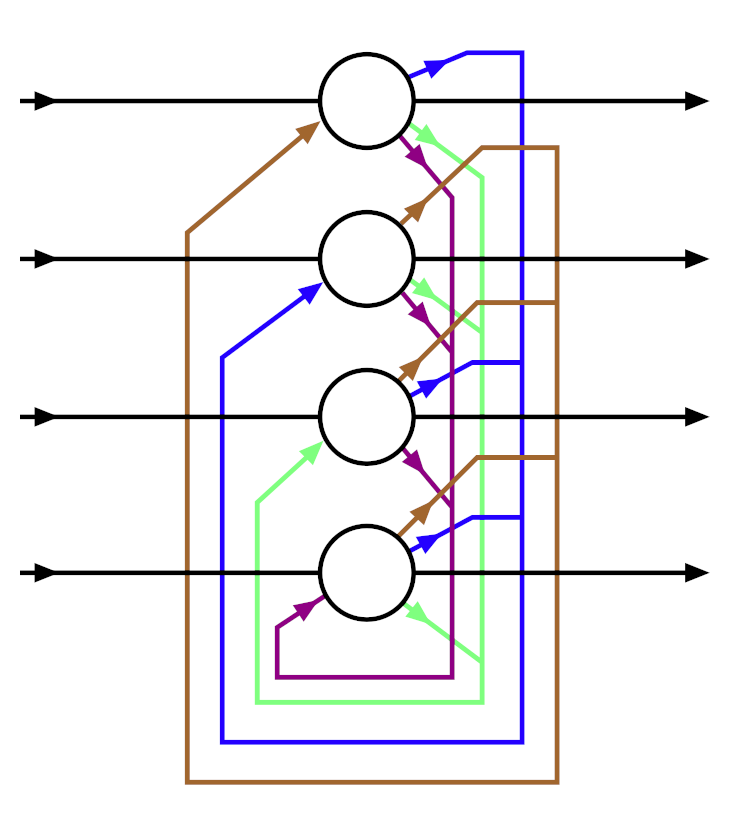
\includegraphics[width=0.95\linewidth]{../img/hopfieldnet.png}
	\caption{Circuit}
	\label{fig:netcircuit}
	\end{subfigure}
	\begin{subfigure}{0.4\textwidth}
		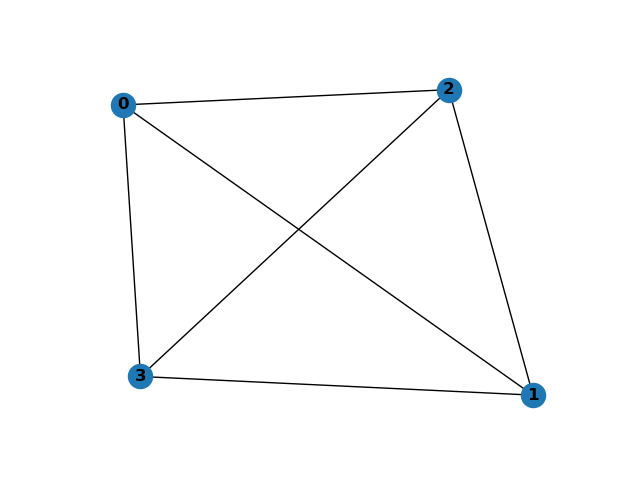
\includegraphics[width=0.95\linewidth]{../img/hopfieldgraph_undirected.png}
	\caption{Graph}
	\label{fig:netgraph}
	\end{subfigure}
	\caption{Two equivalent diagrams of a Hopfield network of 4 nodes}
	\label{fig:net}
	\end{center}
	\end{figure}

	%%%%%%%%%%%%%%% VECTORS	
%	\begin{figure}
%	\begin{center}
%	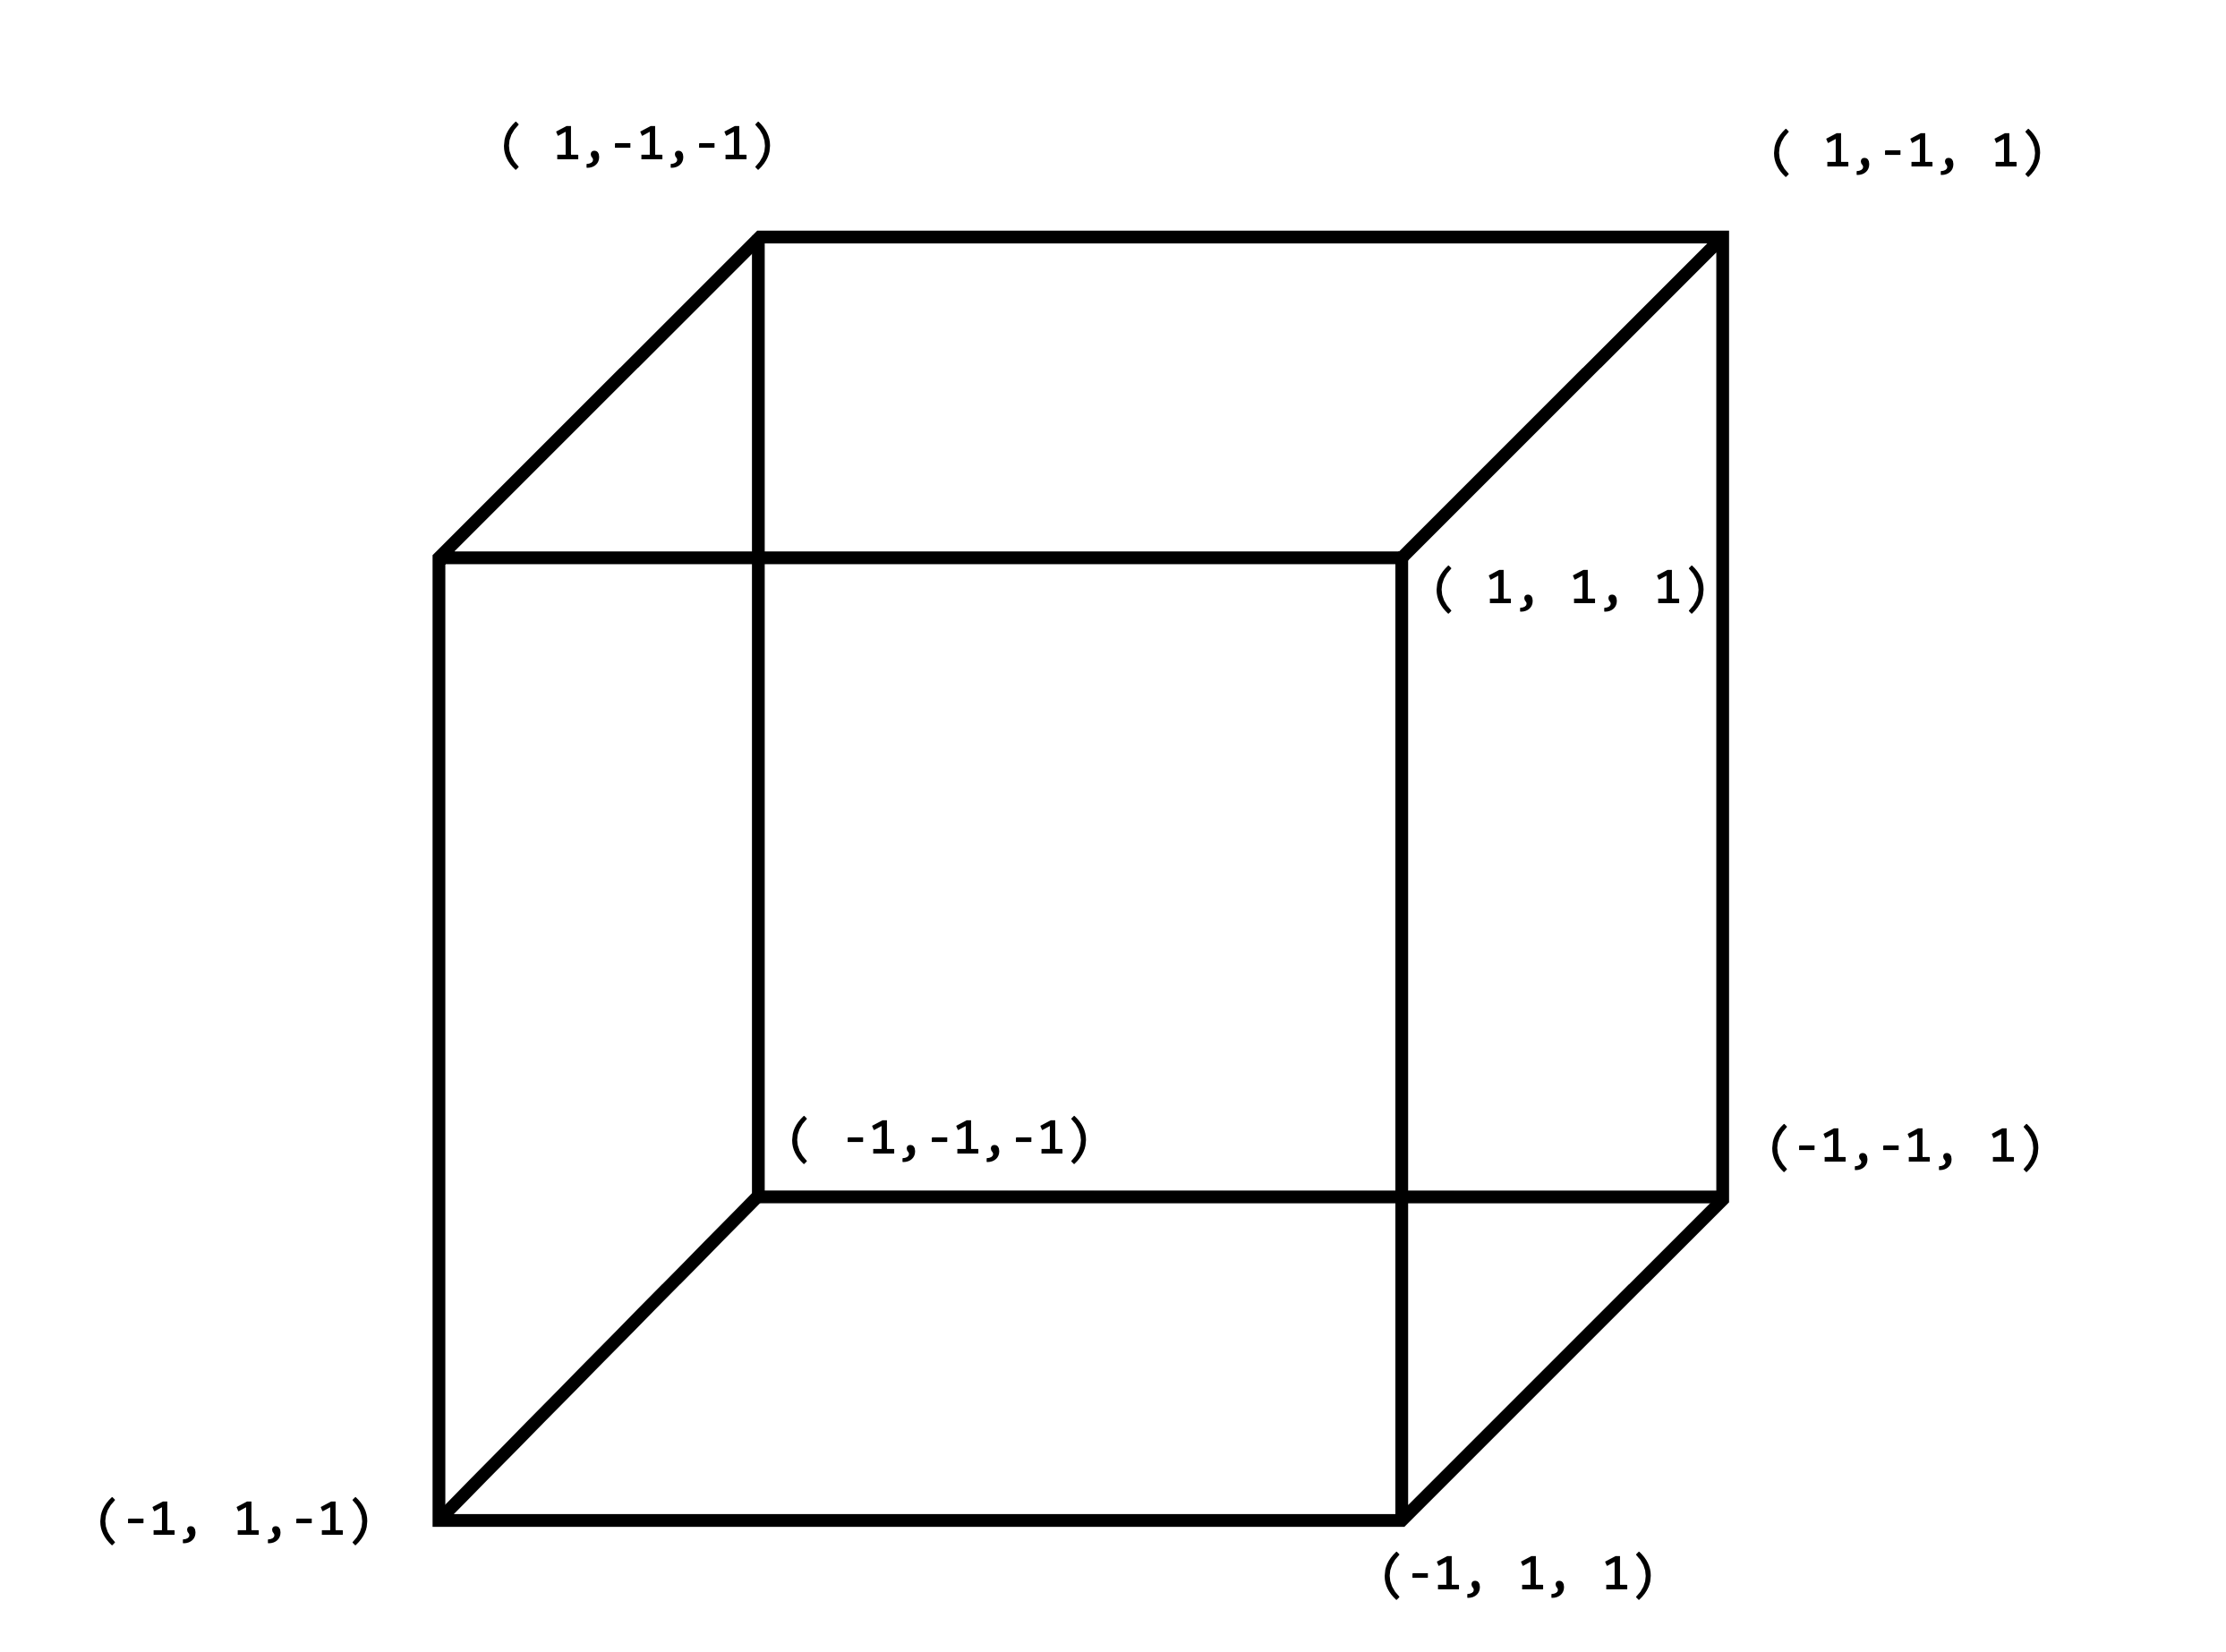
\includegraphics[width=0.4\textwidth]{../img/hypercube.png}
%	\end{center}
%	\caption{Hypercube representation of a three-dimensional binary vector}
%	\label{fig:hypercube}
%	\end{figure}		
	
	\begin{figure}[h!]
	\begin{center}
	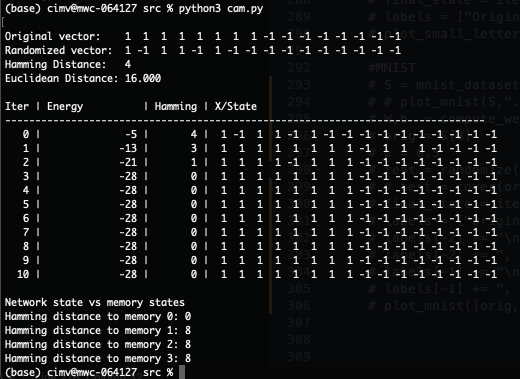
\includegraphics[width=0.75\textwidth]{../img/log_vector_good.png}
	\end{center}
	\caption{HN converging over 10 iterations, N=16, M=4}
	\label{fig:vector_log}	
	\end{figure}

	%%%%%%%%%%%%%.%% LETTERS
	\begin{figure}
	\begin{center}
	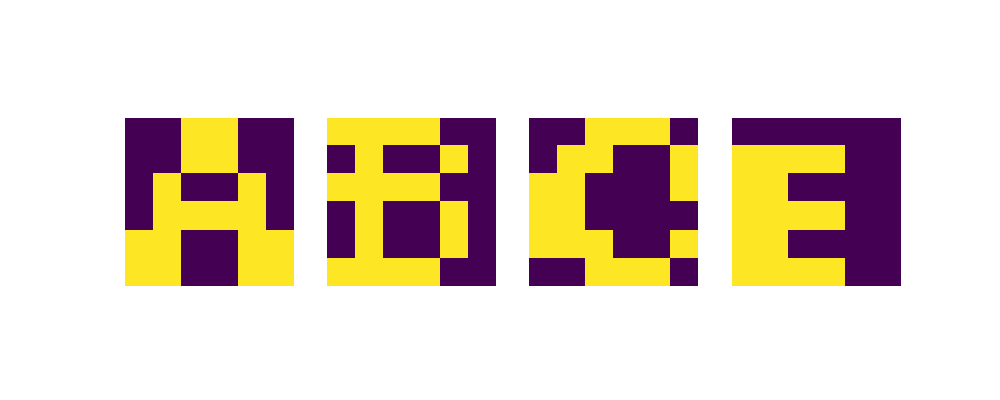
\includegraphics[width=1\textwidth]{../img/small_letters.png}
	\caption{Dataset of 6x6 letters.}
	\label{fig:letters}
	\end{center}	
	\end{figure}

	\begin{figure}
	\begin{center}
	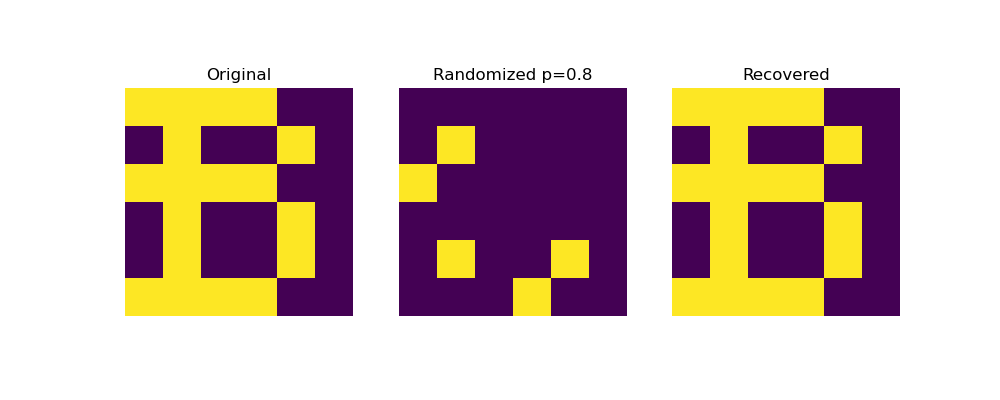
\includegraphics[width=0.8\textwidth]{"../img/letters_result_B.png"} %GOOD 
	\caption{ 6x6 letters. Good convergence in letter 'B'.}
	\label{fig:letters_good}
	\end{center}	
	\end{figure}

	\begin{figure}
	\begin{center}
	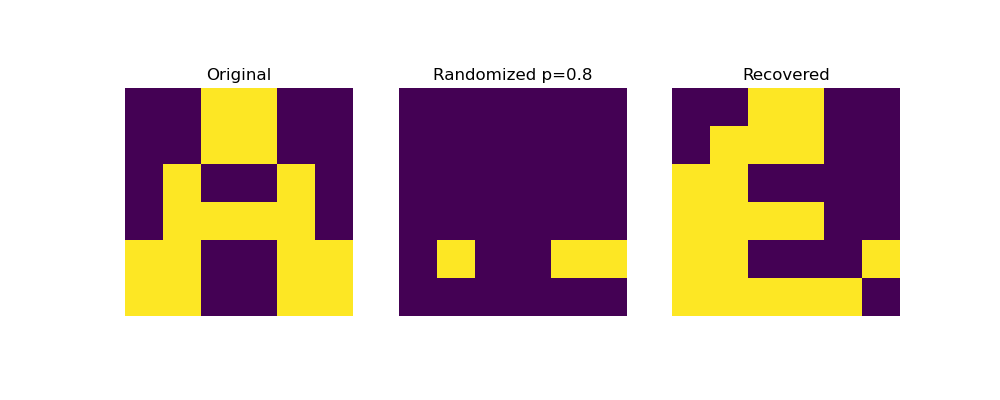
\includegraphics[width=0.8\textwidth]{"../img/letters_result_A.png"}  %BAD
	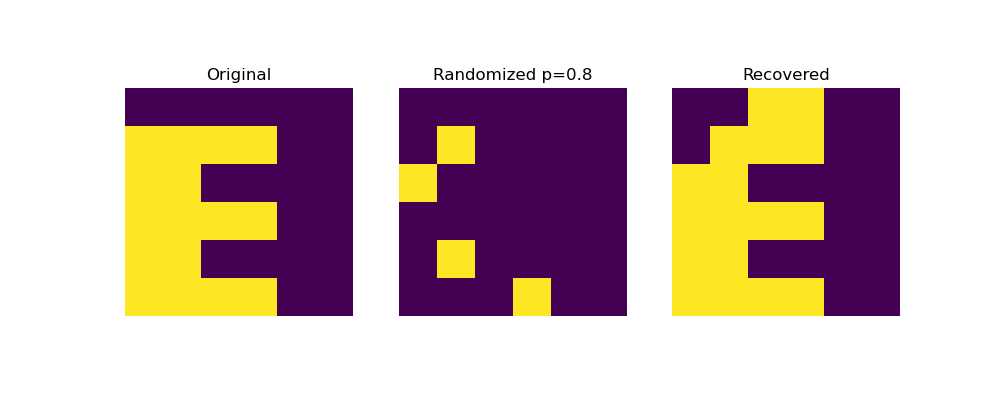
\includegraphics[width=0.8\textwidth]{"../img/letters_result_E.png"}
	\caption{6x6 letters, poor convergence in letters 'A' and 'E'.}
	\label{fig:letters_bad}
	\end{center}	
	\end{figure}

	%%%%%%%%%%%%%%% DIGITS	
	\begin{figure}
	\begin{center}
	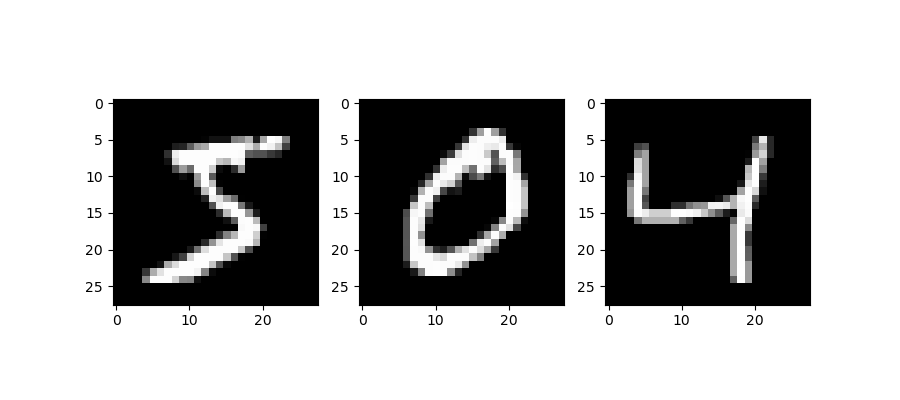
\includegraphics[width=0.8\textwidth]{../img/digits.png}
	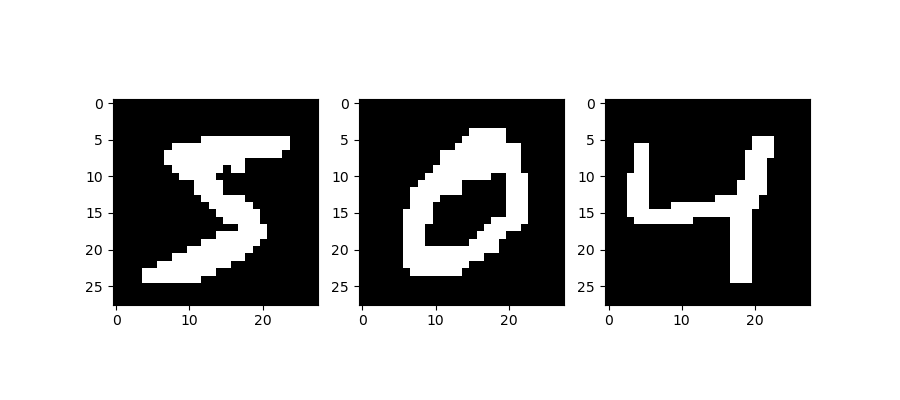
\includegraphics[width=0.8\textwidth]{../img/digits_shifted.png}
	\caption{MNIST dataset of 28x28 grayscale digits. Original grayscale (top), shifted (bottom)}
	\label{fig:digits}	
	\end{center}	
	\end{figure}

	\begin{figure}
	\begin{center}
	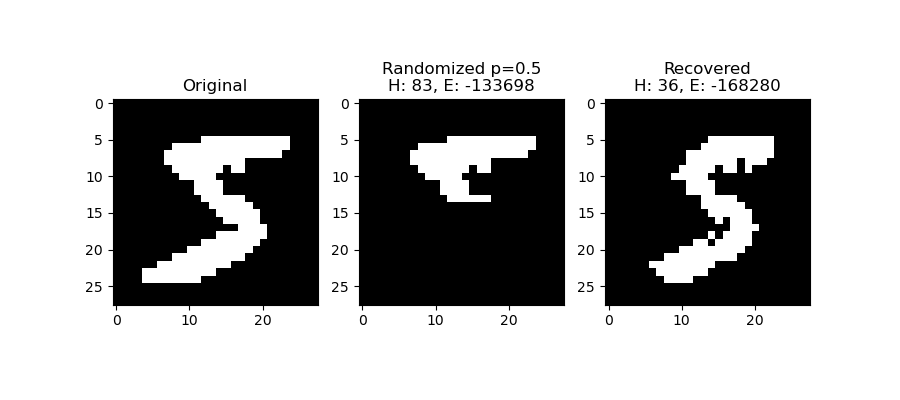
\includegraphics[width=0.75\textwidth]{"../img/digits_result_good_covered.png"}\\
	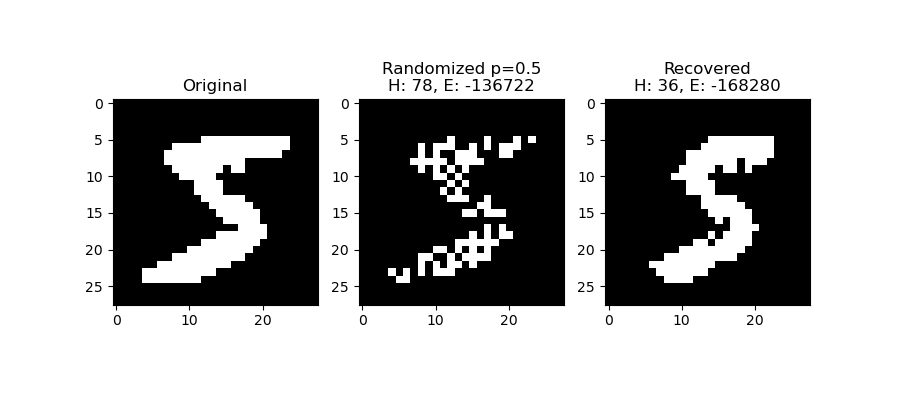
\includegraphics[width=0.75\textwidth]{"../img/digits_result_good_random.png"}
	\caption{MNIST dataset. Good results for digit '5'}
	\label{fig:digits_good}
	\end{center}
	\end{figure}

	\begin{figure}
	\begin{center}
	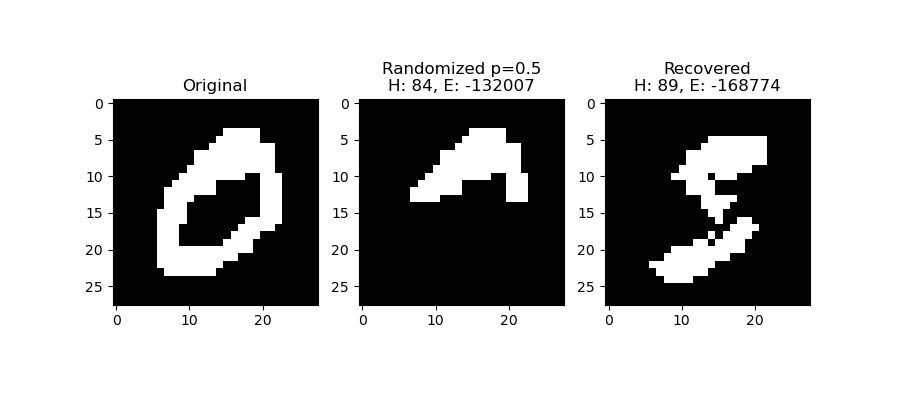
\includegraphics[width=0.75\textwidth]{"../img/digits_result_bad_covered.png"}\\ %BAD
	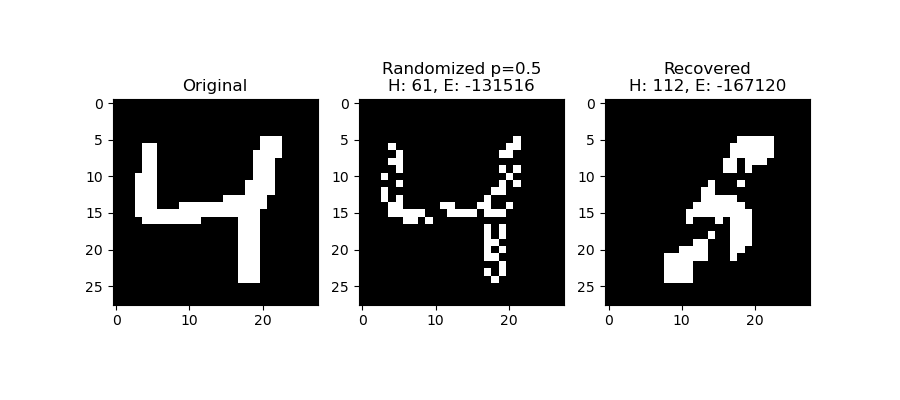
\includegraphics[width=0.75\textwidth]{"../img/digits_result_bad_random.png"}
	\caption{MNIST dataset. Intermediate states for '0' and '4' }
	\label{fig:digits_bad}
	\end{center}	
	\end{figure}
	
\end{document}
